\renewcommand\thetable{\arabic{chapter}-\arabic{table}}
%\renewcommand\thefigure{\arabic{chapter}-\arabic{figure}}
\renewcommand{\theequation}{\arabic{chapter}-\arabic{equation}}
\chapter{校舍耐震資料庫}

學校是人才培育的場所,也是緊急災難時,居民避難的主要地方,但台灣地區學校建築在每次大地震來時之損壞卻非常嚴重,尤其是老舊校舍,因興建年代久遠,其設計所依據之規範較為老舊,耐震能力可能遠低於現今結構耐震安全上之要求,故教育部已委託國家地震工程研究中心進行全國學校校舍之耐震能力評估與補強研究,此計畫建立了校舍建築耐震能力評估補強機制及施行的流程與細節,並且已經對全國學校校舍耐震能力作了全面性的普查,篩選出耐震能力有疑慮之校舍,並儘速透過補強或拆除新建的手段來提昇校舍的耐震能力。而此計畫進行期間所產生之資料,均收集到此一校舍耐震資料庫中。

\section{典型校舍}

我國之校舍建築有極大比例在校舍的結構形式、幾何尺寸等都有相似的結構,其平面配置多如圖~\ref{fig:TSB},這類校舍都為一字型的長形建築,教室一間接著一間排列,教室外有走廊,走廊外多有柱,且樓層數不超過五樓,這一種常見的校舍在教育部的耐震能力補強計畫中統稱為「典型校舍」,典型校舍在受到地震力作用時且造成破壞時,破壞的樓層通常都在一樓,而且是沿著一字形的長邊的方向破壞。由於典型校舍通常的破壞模式為沿著校舍的長向破壞,也就是走廊的方向,因此側推分析所施加的側力也就是沿著長向施加,而長向也被稱為~X~向,另外一個方向,也就一字形較短的那一邊,則是~Y~向,而施加力量的方向則是正向,和力量相反的方向則是反向。

\begin{figure}[hbtp]
  \begin{center}
    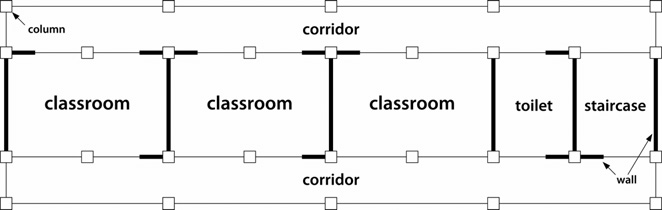
\includegraphics[width=1.0\textwidth]{figures/trad-school-buildings.png}
    \caption{典型校舍} 
    \label{fig:TSB}
  \end{center}
\end{figure}

典型校舍因為其結構形式單純,只需要少量的屬性便可以完整的描述建築物的結構,不用完整詳細的記錄所有的樑柱等構件之個別尺寸強度與位置到可以建立數值模型的程度,因屬性數量較少,其校舍資料很適合進行各種資料分析的研究。

\section{收集範圍}

校舍的耐震能力補求流程如圖~\ref{fig:FLOW}~所示。可以分為四個大步驟,分別是校舍普查、初步評估、詳細評估、補強設計與施工,校舍普查主要之目的為全國所有校舍之基本資料建檔,並簡單調查一些主要的設計參數,是由~NCREE~主導進行,其性質類似於人口普查,是整個計畫中非常重要的基礎建設;接著第二個步驟的初步評估則是根據於校舍普查之基礎,對校舍進行初步評估(preliminary evaluation),其通常的方法是基於結構物之設計及現況填寫評估表,所填寫資料再依評估公式計算出結構物耐震能力之評分等級或指數,此類方法之評估速度快,但是結果可靠度較低,主要的目的是對大量結構物之耐震能力作排序與篩選,這類型評估方法所使用之評估表與評估公式通常是使用已經收集的其他結構物資訊,用數值統計的方法迴歸,或是根據基本的結構耐震能力供需比以及專業人士相關的經驗設計得到的,其所適用之結構物類型也有所限制,評估表並不能套用到各種類型的結構物上;接著經過初步評估後,對於耐震能力有疑慮之校舍,需要進一步進行詳細評估(detailed evaluation),此類方法為對結構物進行詳細的結構耐震分析,通常是使用結構分析程式以電腦數值模擬結構物遇到地震時的非現性行為,並根據模擬結果為依據,準確詳細的檢驗評估出結構物的耐震能力;詳細評估之後,才根據技師的專業判斷,對於耐震堪慮之校舍,依嚴重程度,由工程專業人員,進行結構耐震之詳細評估,倘尚符合補強之經濟效益,即進一步作耐震補強之設計,若不符合補強之經濟效益,則將之列為拆除重建。


\begin{figure}[hbtp]
  \begin{center}
    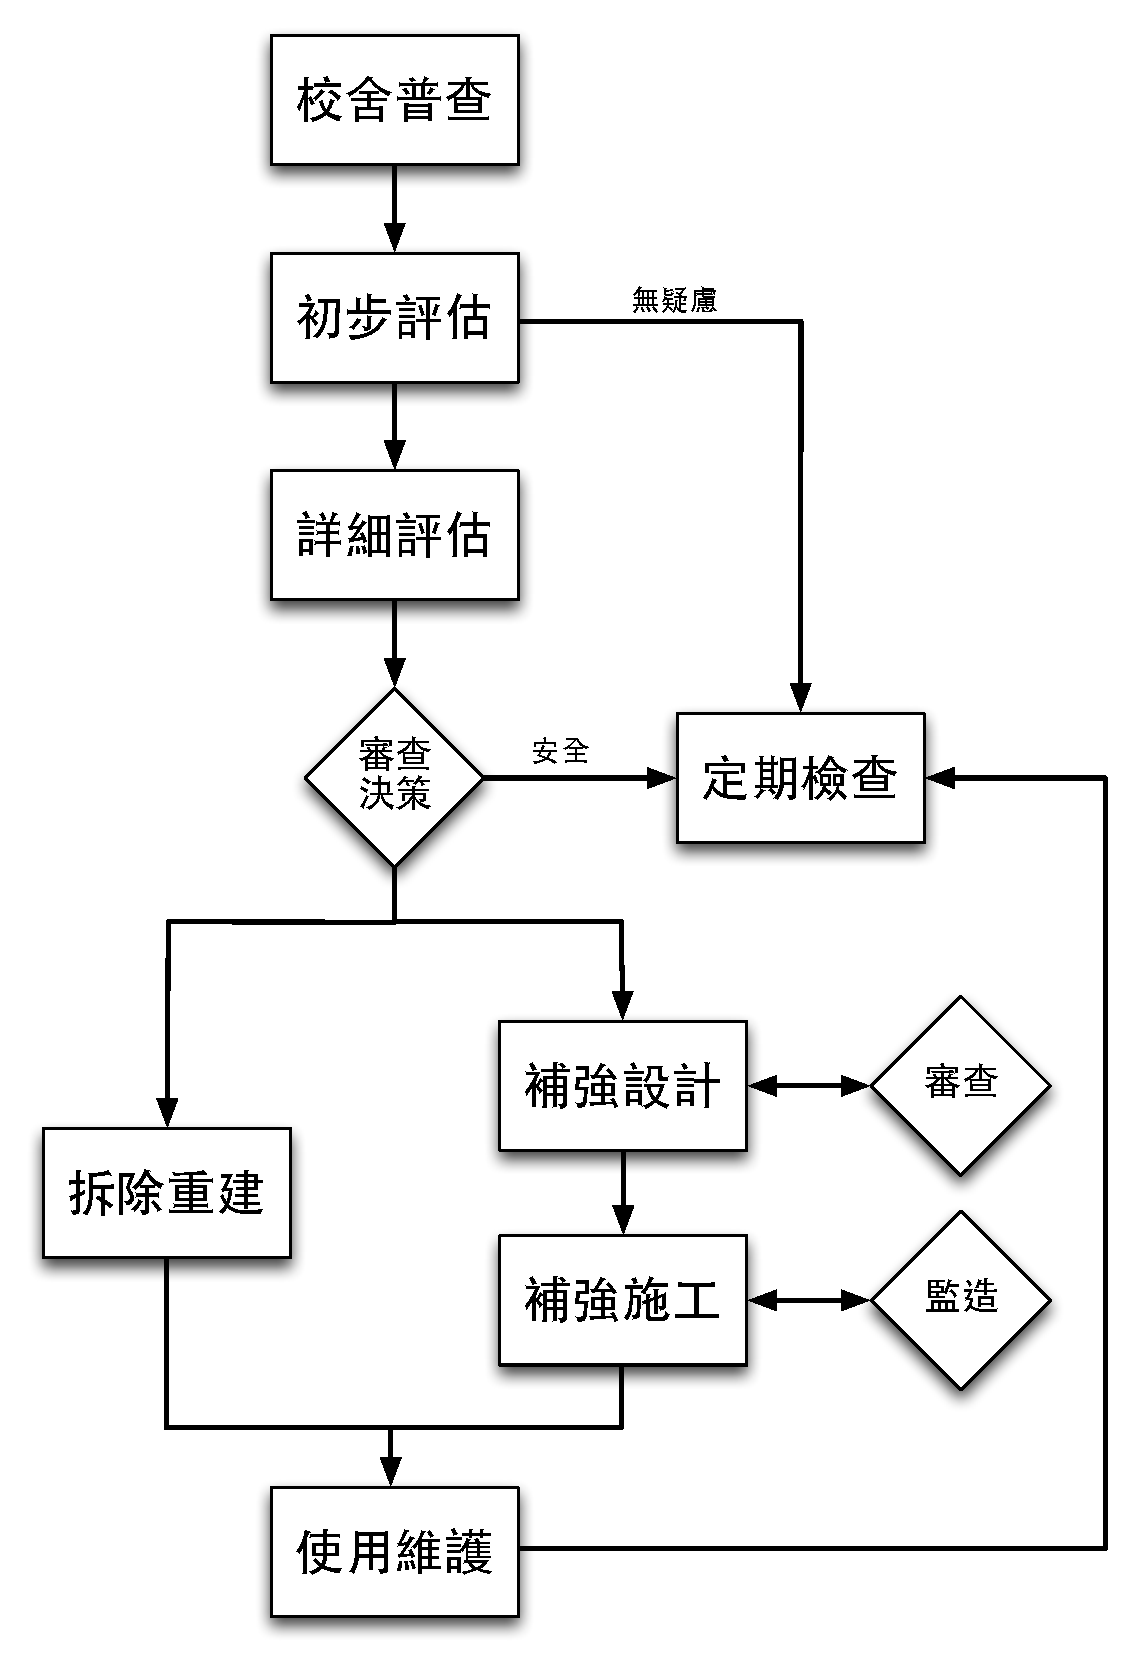
\includegraphics[width=\textwidth]{figures/survey-flow.pdf}
    \caption{評估流程} 
    \label{fig:FLOW}
  \end{center}
\end{figure}

詳細評估方法的可靠度較高,但是花費相當昂貴,所需要的時間也比使用評估表要來的久很多,由於中小學校舍數量龐大,若直接大量投入人力物力,可能造成大量之資源浪費,也無法快速的鎖定耐震能力不足之校舍建築,故針對有效達成此一校舍耐震評估標準需求以及基於上述標準耐震評估程序之精神,NCREE~才提出先經由初步評估方法進行篩選的分段式評估方法,有效的將校舍結構之耐震能力排序,以縮小問題之規模,提升整體校舍耐震能力評估作業的效率。

在此過程中會產生的校舍資料最重要的為:初步評估、詳細評估、補強設計、補強工程等四組資料,以下分別介紹四組資料之背景原理及所收集的資訊。

\subsection{初步評估}

詳細評估的原理是分別求取結構物對於地震的需求(demand)和可以承受地震的能力(capacity),然後取其比值,也就是耐震需求比($CDR$),如果耐震需求比大於~1~則表示建築物的耐震能力足夠,足以承受未來可能發生的大地震。而初步評估雖然是簡化的評估方法,但其原理也和詳細評估相同,是以求得結構物的耐震需求以及耐震能力的比值為目標,耐震需求的部分,是以校舍所在地,可能發生的~475~年週期之最大地震力作為其所需要承受之地震力。至於耐震能力是根據結構物的載重元件尺寸例如牆、柱之斷面積,以及~NCREE~歸納之公式所推算得到之強柱等效強度,求得之值校舍之基本耐震性能~$E$,求得~$E$~後,還要根據校舍現況及專業人士判斷做調整,最後得到之耐震指標為~$Is$~,其是一個百分制系統,如果~$Is = 100$~則等同於~$CDR = 1$~,表示結構物之耐震能力與需求相同。



%初步評估相較於詳細評估的模擬運算而言,是簡化許多的耐震能力評估方式,評估的方式是使用地震中心根據過往資料與相關規範所設計而得,其設計的基礎與詳細評估的 $CDR$ 值相同,皆為校舍的耐震能力與耐震需求的比值,主要的對象為典型校舍,假設校舍之破壞位置為長向的一樓,耐震需求為則為建築物需要能承受其所在地所可能發生的的475年週期最大地震之地震力,由推估的校舍載重以及地震之地表加速度推估而得。而耐震能力則是根據校舍之柱、牆等尺寸,並根據實驗數據推估所得到的等效強度,兩者相除後再乘上調查人員根據校舍現況所填入之調整參數 $Q$,所得到的 $Is$ 即為使用初步評估表格所評估之校舍耐震能力。

\subsection{詳細評估}

美國針對鋼筋混凝土(RC)建築物之耐震能力規範ATC-40\cite{applied1996seismic}中,建議用來評估建築物耐震能力之方法稱為容量震譜法(capacity spectrum method),此一評估方法可以分為兩個部分,第一部分是進行側推分析(pushover analysis)取得容量震譜(capacity spectrum),流程如Figure 1所示,第二部分是根據建築物所在地的各種相關資訊和規範取得需求震譜(demand spectrum),接著使用容量震譜法(capacity spectrum method)以取得建築物性能點,根據性能點(performance point)座標帶入公式計算可以得到建築物的破壞地表加速度(collapse ground acceleration)以及耐震能力指標(aseismic ability index),如Figure 2所示。

求取容量震譜的側推分析(pushover analysis)需要先建立建築物完整的非線性分析模型(nonlinear structure model),此模型要由進行評估的專業人士根據建築物的幾何尺寸資訊來建立基本的建築物框架。接著根據建築物的材質計算建築物自身重量以及需要承載的人員和配設物件之重量,並將其附加到柱、牆等承載元件上。接著最重要的是設定建築物各構成元件如樑、柱、牆受力時的非線性行為,這些力與變形的關係多為實驗得到或是利用其他分析模擬方法得到的。至此,側推分析(pushover analysis)要用的數值模型才算建立完成。而側推分析(pushover analysis)其程序是依照規範,使用建議之側力,逐步地給結構模型施加增量外力,將結構物向某一方向推動,每次增量即進行一次結構分析計算每一構件之應力(stress)與變位(strain),之後與上一次的分析結果累加即可得到每一個構件於此受力階段之反應,並判斷構件是否破壞,例如開裂(crack)、降伏(yield),甚至達到極限強度(ultimate force)等,之後各構件依其破壞程度更新其行為,例如改變其勁度,或者將已發生破壞的構件從結構模型中抽離,如此重複分析直到結構不穩定而崩垮為止,側推分析完成後可以得到建築物之容量震譜(capacity spectrum)。

需求震譜(demand spectrum)是根據建築物環境現況,參考規範製成之地震需求頻譜。參考的環境狀況如土層種類,堅硬的土層可以讓建築物有較好的抗震能力。另外靠近斷層的建築物在地震發生時往往會因為斷層於地震時產生的反應而受到嚴重的損害,因此建築物與斷層的距離也納入參考的資料之一,稱為近斷層效應(special effects of near-source earthquakes),其他還需要的資料有地層資料、地震震區等,綜合這些資料並參考規範即可得到該建築物所需符合之需求震譜。

容量震譜法(capacity spectrum method)最後是將需求震譜(demand spectrum)以及容量震譜(capacity spectrum)轉換格式後相疊,求取建築物之性能點(performance point),性能點之物理意義為該建築物在特定水準地震下所能承受之最大變位(strain)及剪力(shear force),但是由於結構物受地震力作用進入非線性行為時,結構物的阻尼效應會產生消能的作用,因此還要視情況對需求曲線進行折減,此為一個迭帶運算的過程,可能需要不斷折減需求曲線,並進行性能點(performance point)正確性的檢核,直到檢核通過,才能得到建築物真正之性能點(performance point)如Figure 2 (d),由建築物性能點(performance point)之座標帶入公式可以求得建築物的破壞地表加速度(collapse ground acceleration)$A_C$,詳細評估所使用的耐震能力值為 $CDR$,其定義如下:

\begin{equation} CDR = \dfrac{A_C}{A_D} \label{eq:CDR}\end{equation} 

$A_D$ 為根據建築物所在地的並依據規範所得到的,建築物所需要能承受的475年週期最大地震所產生之地表加速度,$CDR$大於~1~代表此一棟建築物能夠承受該地區475年一遇的最大地震。

\subsection{補強設計}

ask 趙哥

如果校舍經過詳細評估過後,負責的專業人士認為此棟校舍確實有安全疑慮,但尚可以補強,不需要拆除重建時,則該棟校舍需要進入補強設計,補強設計階段中,負責的專業人士需要依據詳細評估的結果,設計出兩種不同的補強方案,並且對不同的補強方案進行詳細的耐震能力評估,因此這個階段的資料包括兩組補強設計的資料,以及兩組補強後的耐震能力詳細評估資料。補強設計收集的資料主要為使用的補強工法以及補強量,主要收集的補強工法包括了:擴柱、剪力牆等,

\subsection{補強工程}

ask 趙哥

補強工程部分的資料則包括了實際補強工程的相關資料,其中包括了採用的補強設計,工程發包的相關資料,例如工程經費、發包時間、驗收報告等等。